\chapter{Malware}

\textit{Un programma che viene inserito in un sistema (solitamete di nascosto) 
con l'intento di compromettere la riservatezza, integrità o disponibilità dei dati.}

Il codice malevolo si comporta in modo inaspettato, grazie all'iniziativa di 
un programmatore malizioso.

\section{Classificazione}

I malware possono essere classificati:
\begin{itemize}
    \item sulla base della propagazione (legati ad altro software, rete, social engeneering, \dots)
    \item azioni del payload (corruzione di dati, furto di dati)
    \item motivazione/attori dell'attacco 
\end{itemize}

\begin{figure}[ht]
    \centering
    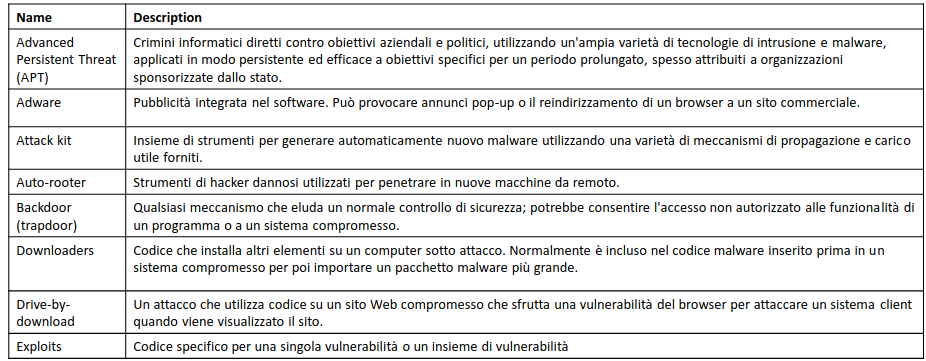
\includegraphics[width=1\linewidth]{chapters/images4/term1.png}
\end{figure}
\begin{figure}[ht]
    \centering
    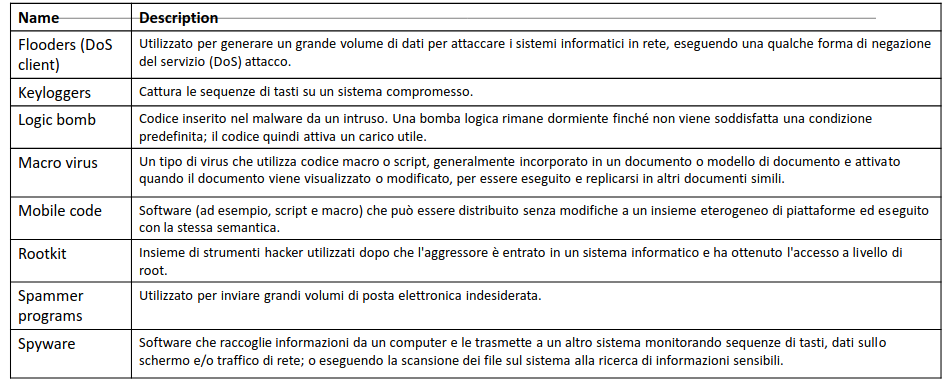
\includegraphics[width=1\linewidth]{chapters/images4/term2.png}
\end{figure}
\begin{figure}[ht]
    \centering
    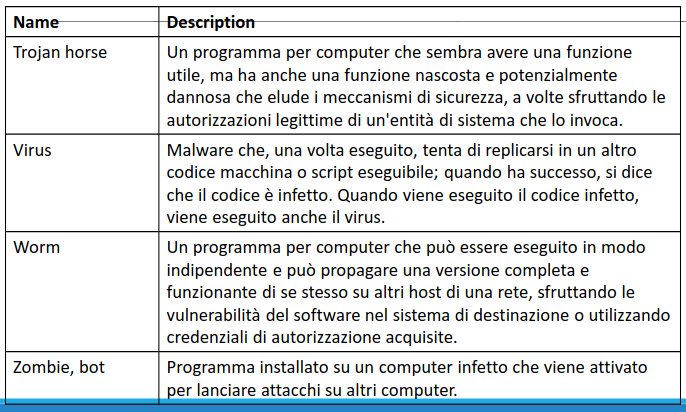
\includegraphics[width=1\linewidth]{chapters/images4/term3.png}
\end{figure}

\section{Virus}

Un virus informatico è un codice informatico che
può replicarsi modificando altri file o programmi
per inserire codice in grado di essere replicato
ulteriormente.

La \textbf{proprietà della replicazione} è ciò che distingue i virus
informatici da altri tipi di malware.

Un'altra proprietà dei virus è che la replica richiede \textbf{richiede un
certo tipo di assistenza da parte dell'utente} (cliccare su un allegato email, \dots).

I virus cercano sempre di rimanere nell'ombra.

\subsubsection{Composizione dei virus}
Generalmente i virus sono composti da tre parti:
\begin{itemize}
    \item \textbf{meccanismo di infezione}
    \item \textbf{trigger}, cioè l'evento che determina quando il payload viene attivato; è conosciuto anche come \textbf{bomba logica}
    \item \textbf{payload}, cioè cosa fa il virus
\end{itemize}

\subsubsection{Fasi di un virus}
I virus attraversano quattro fasi:
\begin{enumerate}
    \item \textbf{fase dormiente:} il virus deve ancora essere attivato
    \item \textbf{fase scatenante:} il virus viene attivato per svolgere la funzione per la quael era previsto
    \item \textbf{fase di propagazione:} il virus inserisce una copia di sé stesso in altri programmi o aree del disco; ogni programma conterrà 
    un clone del virus che entrerà a sua volta in fase di propagazione
    \item \textbf{fase esecutiva:} la funzione viene eseguita
\end{enumerate}

\subsection{Macrovirus}

Virus che si attaccano ai documenti dell'utente.

Sono minacciosi per una serie di motivi:
\begin{itemize}
    \item è indipendente dalla piattaforma
    \item infetta i documenti, non porzioni di codice
    \item si diffondono facilmente
    \item più facili da scrivere
\end{itemize}

\subsection{Classificazione dei virus}
I virus possono essere classificati secondo i meccanismi che utilizzano per 
non essere rilevati:
\begin{itemize}
    \item \textbf{encrypted virus:} una parte del virus crea una chiave casuale con cui cripta il resto del virus; questa chiave viene
    usata per decriptare quando un viene chiamato il programma infetto. Per evitare attacchi di frequenza ogni volta che il virus 
    si replica viene usata una chiave diversa
    \item \textbf{stealth virus:} progettati per nascondersi dagli antivirus, usando tecniche di mutazione del codice o compressione
    \item \textbf{polymorphic virus:} durante la replica crea copie con la stessa funzionalità ma hanno modelli di bit diversi 
    \item \textbf{metamorphic virus:} si riscrive completamente ad ogni iterazione, aumentando la difficoltà di rilevamento
    \item \textbf{compression virus:} comprimono il file eseguibile in modo che sia la versione infetta che quella non infetta abbiano la stessa lunghezza
\end{itemize}

\section{Worm}

Software analoghi ai virus ma che non hanno bisogno di un programma benigno a cui attaccarsi, ma agiscono da soli.

Hanno lo stesso funzionamento e fasi dei virus.

Attualmente i worm cercano di spaziare su più piattaforme possibili, cercando più vulnerabilità
e diffondendosi velocemente. Utilizzano tecniche di polimorfismo e metamorfismo.

\section{Drive-by-downloads}
Sfruttano dei bug nelle applicazioni utente per installare malware.

Una tecnica comune sfrutta le vulnerabilità del browser: quando un utente visita un pagina web controllata
dall'attaccante, scarica e installa un malware a sua insaputa sfruttando dei bug.

Questo malware attende che utenti ignari visitino la pagina Web dannosa per diffondersi sui loro
sistemi.

\section{Clickjacking}

L'attaccante raccoglie i click dell'utente e lo costringe a fare una varietà 
di cose, come ad esempio:
\begin{itemize}
    \item indirizzare a siti web che contengono codice dannoso
    \item viene posizionato un pulsante sotto ad un'altro ad insaputa dell'utente
    \item i click della tastiera vengono dirottati (l'utente crede di digitare da una parte ma invece 
    digita in una porzione controllata dall'attaccante)
\end{itemize}

Si tratta sostanzialmente di dirottare i click dell'utente, utilizzando
i diversi livelli di una pagina web.

\section{Zombie \& Botnet}
Prende il possesso segretamente di un altro computer sfruttando i 
difetti del software; viene usata per lanciare indirettamente altri attacchi:
\begin{enumerate}
    \item viene creata la rete di botnet; scansiona internet cercando di capire quali sono gli host che possono essere attaccati
    \item l'attaccante installa dei \textit{zombie agent}, ovvero dei programmi installati da remoto che danno il controllo della macchina
    \item gli zombie agent fanno riferimento ad un \textit{master}, che controlla il funzionamento della rete di macchine
    \item l'attaccante dà un comando che verrà eseguito da tutte le macchine infette (DDoS, spam, keylogging, sniffing, \dots)
\end{enumerate}

\section{Rootkit}
Sono dei programmi che dà remoto danno l'accesso di root, dando il controllo del sistema. Superano
i normali controlli di autenticazione.

Possono essere installati a diversi livelli (applicazione, kernel).

\section{Spear Phishing}
Vengono inviate mail a particolari target (impiegati di una società, \dots); 
dopo aver studiato la vittima, e facendo affidamento al social engeneering per 
far apparire le email in modo convincente.

Risulta più difficile individuare questo tipo di email fasulle, sono molto
mirate alla singola vittima/compagnie.


\section{Approcci alle contromisure per i malware}
Dovrebbero essere adottate diverse contromisure, come:
\begin{itemize}
    \item assicurarsi che tutti i sistemi siano aggiornati, per ridurre il numero di vulnerabilità
    \item impostare controlli di accesso alle applicazioni e ai dati nel sistema, per limitare il numero di file a cui ogni utente può accedere, e
    di conseguenza che può infettare o corrompere
\end{itemize}

Esistono diverse azioni di mitigazione delle minacce:
\begin{itemize}
    \item \textbf{rilevamento:} accertarsi della sua esistenza e rilevare il malware
    \item \textbf{identificazione:} individuare lo specifico malware 
    \item \textbf{rimozione:} rimuovere tutte le tracce del malware in modo che non possa diffondersi ulteriormente
\end{itemize}




